\documentclass[conference]{IEEEtran}
\IEEEoverridecommandlockouts

\usepackage{cite}
\usepackage{amsmath,amssymb}
\usepackage{booktabs}
\usepackage{array}
\usepackage{algorithm}
\usepackage{algorithmic}
\usepackage{graphicx}
\usepackage{tikz}
\usetikzlibrary{arrows.meta,positioning,fit,calc,shapes.geometric}
\usepackage{url}
\usepackage{xcolor}
\usepackage{listings}

\lstdefinestyle{solidity}{
  basicstyle=\ttfamily\scriptsize,
  breaklines=true,
  columns=fullflexible,
  frame=single,
  numbers=left,
  numberstyle=\tiny,
  xleftmargin=1.2em,
  numbersep=0.4em,
  keywordstyle=\color{blue!60!black},
  morekeywords={contract,function,mapping,uint,address,public,external,payable,require,if,bool,return,modifier}
}

\newcommand{\tool}{\textsc{HyperVul}}
\newcommand{\pct}[2]{$#1 \pm #2$}

\begin{document}

\title{\tool{}: Safety-Aware Hypergraph Interaction Modeling for Smart Contract Reentrancy Detection}

\author{
\IEEEauthorblockN{Anonymous Author(s)}
\IEEEauthorblockA{
\textit{Anonymous Institution}\\
Anonymous City, Country\\
anonymous@email.edu}
}

\maketitle

\begin{abstract}
Existing AI-based smart contract vulnerability detectors commonly model programs as token sequences, functions, or pairwise program graphs. However, vulnerabilities such as reentrancy are higher-order phenomena: they arise from the joint presence of an externally callable function, a sensitive state variable, an external call, unsafe state-update ordering, and missing protection. Pairwise graph edges fragment this $n$-ary relation into isolated binary signals, forcing models to infer vulnerability semantics indirectly and contributing to false positives on protected reentrancy-like code.

This paper presents \tool{}, a safety-aware hypergraph learning tool for smart contract vulnerability detection and localization. \tool{} represents vulnerability-relevant behavior as interaction hyperedges that jointly encode function context, state access, external calls, callees, call type, and security evidence. It performs contract-level detection while ranking suspicious interactions for top-$k$ localization. To reduce false positives, \tool{} explicitly separates risk evidence from safety evidence, including reentrancy guards, safe wrappers, guard conditions, access-control evidence, and state-update order.

We evaluate \tool{} on reentrancy detection against function-level, sequence-based, call-graph, and pairwise graph neural baselines. Experimental results show that \tool{} improves contract-level vulnerability detection and produces accurate ranked localization of suspicious interactions, achieving 64.34 contract-level F1, 82.50\% Top-1 localization, 96.25\% Top-3 localization, and 90.42\% MRR. These results suggest that safety-aware hypergraph interaction modeling is a practical AI-tool direction for improving both vulnerability detection and explanation quality in smart contract analysis.
\end{abstract}

\begin{IEEEkeywords}
smart contract security, reentrancy detection, hypergraphs, vulnerability localization, graph neural networks
\end{IEEEkeywords}

\section{Introduction}

Smart contracts are programs deployed on blockchains to manage assets, enforce financial logic, and coordinate decentralized applications. Their security failures can be costly because contract execution is public, adversarial, and difficult to patch once deployed. Automated vulnerability detection is therefore an important application area for AI-based software engineering tools.

Existing smart contract analyzers can be grouped into two broad families. Rule-based and symbolic tools, such as Oyente~\cite{luu2016oyente}, Securify~\cite{tsankov2018securify}, SmartCheck~\cite{tikhomirov2018smartcheck}, and Slither~\cite{feist2019slither}, provide practical static analysis for known bug patterns. Learning-based detectors instead represent code as tokens, functions, or program graphs, and train classifiers to predict vulnerabilities from labeled examples~\cite{zhuang2020gnn}. These systems have advanced automated analysis, but they often struggle with two related problems: high false-positive rates and limited localization of the actual vulnerable behavior.

The core limitation we study is a representation mismatch. Many graph-based detectors encode programs using pairwise edges, such as control-flow, data-flow, call, or dependency relations. Pairwise graphs are useful for general structure, but they are not always aligned with the semantics of vulnerabilities. A reentrancy bug, for example, is not caused by an external call alone. It arises from an $n$-ary condition involving a function, an accessed state variable, an external call, the callee, the relative order of state updates, and the absence of an effective guard. When this relation is decomposed into separate binary edges, the model must reconstruct the vulnerability indirectly from fragmented signals.

Figuratively, the vulnerable unit is the interaction:
\begin{equation}
(f,\; s,\; e,\; c,\; o,\; g),
\end{equation}
where $f$ is the function context, $s$ is a sensitive state variable, $e$ is an external call, $c$ is callee evidence, $o$ describes ordering, and $g$ represents guard or protection evidence. Pairwise encodings split this relation into isolated edges such as $(f,s)$, $(f,e)$, and $(e,c)$, and often represent missing guards only implicitly.

This paper presents \tool{}, a safety-aware hypergraph learning tool for reentrancy detection and localization. \tool{} builds interaction hyperedges that connect the relevant entities of a candidate vulnerability pattern. Instead of training only an interaction-level classifier, \tool{} performs contract-level detection using multiple-instance learning (MIL): a contract is represented as a bag of candidate interactions, and the model predicts whether at least one interaction is vulnerable. At the same time, the interaction scores provide ranked explanations for top-$k$ localization.

The paper makes the following contributions:
\begin{itemize}
    \item We define reentrancy detection as a higher-order interaction problem and show why pairwise program graphs fragment the $n$-ary security condition that determines vulnerability.
    \item We introduce \tool{}, a safety-aware hypergraph architecture that jointly models function context, state access, external calls, callees, update order, and protection evidence for contract-level detection and interaction localization.
    \item We provide a reentrancy-focused evaluation against function, sequence, call-graph, and pairwise graph baselines, including top-$k$ localization and ablations of contract-level training, safety-aware modeling, and targeted reentrancy training.
\end{itemize}

\section{Related Work}

\subsection{Static Smart Contract Analysis}
Early smart contract vulnerability detection relied heavily on symbolic execution and static rules. Oyente introduced symbolic execution for Ethereum contracts and detected patterns such as reentrancy and transaction-ordering dependence~\cite{luu2016oyente}. Securify used compliance and violation patterns to reason about contract safety properties~\cite{tsankov2018securify}. SmartCheck translated Solidity code into an XML-based intermediate representation and applied XPath-style rules~\cite{tikhomirov2018smartcheck}. Slither introduced a practical static analysis framework and an intermediate representation for Solidity~\cite{feist2019slither}. These tools are useful in audit workflows, but rule-driven analyzers may over-report risky-looking but protected code, especially when the safety condition depends on context.

\subsection{Learning-Based Vulnerability Detection}
Learning-based tools attempt to generalize beyond hand-written rules by training classifiers over code representations. Sequence models treat source code as text or tokens; feature-based models aggregate hand-crafted security indicators; graph neural networks learn over program graphs. These approaches reduce manual rule engineering, but they inherit the limitations of their representation. A function-level classifier may know that a function contains an external call, but it may not distinguish whether the relevant state update happens before or after the call. A sequence model may observe syntax order, but it lacks explicit relations among state variables, callees, and guards. A pairwise graph model captures local edges but fragments higher-order vulnerability conditions.

\subsection{Graph and Higher-Order Program Representations}
Graph neural networks such as GCNs~\cite{kipf2017gcn}, GATs~\cite{velickovic2018gat}, and relational GCNs~\cite{schlichtkrull2018rgcn} have been used for many structured prediction tasks, including program analysis. In smart contract security, graph-based detectors typically encode AST, CFG, data-flow, or call-graph relations~\cite{zhuang2020gnn}. However, reentrancy depends on a joint configuration of multiple program entities. Hypergraphs provide a natural way to represent such higher-order relations because a hyperedge can connect more than two entities. \tool{} uses this idea to make the candidate vulnerability interaction itself the model's prediction and explanation unit.

\section{Problem Formulation}

\subsection{The Representation Gap}

Let a smart contract be denoted by $C$. A learning-based detector first maps $C$ into a representation $\rho(C)$ and then learns a scoring function over that representation. The choice of $\rho$ is not neutral: it defines which program relations are easy or hard for the model to express. Token and sequence models define $\rho(C)$ as ordered text; function models define it as a set of function embeddings; conventional graph models define it as a pairwise program graph:
\begin{equation}
G_C=(\mathcal{V}_C,\mathcal{E}_C),
\end{equation}
where $\mathcal{V}_C$ contains program entities and each edge $(u,v,r)\in\mathcal{E}_C$ is a typed binary relation, such as calls, reads, writes, controls, or depends-on.

Pairwise graphs are expressive for local structural facts, but they impose a binary factorization on security conditions that are often not binary. Reentrancy is the central example considered in this paper. The vulnerable behavior is not the external call alone, nor the state variable alone, nor a function name alone. It is the joint configuration:
\begin{equation}
\Psi(f,S,e,c,o,g)=1,
\end{equation}
where $f$ is the function context, $S$ is the set of sensitive state variables, $e$ is an external call site, $c$ is callee evidence, $o$ describes state-update ordering relative to the call, and $g$ denotes effective protection evidence such as guards or modifiers.

A pairwise graph represents this condition only through a projection:
\begin{equation}
\pi(\Psi)=\{(f,S),(f,e),(e,c),(f,g),(S,o),(e,o)\}.
\end{equation}
This projection preserves individual binary facts, but it loses the fact that these facts jointly form one candidate vulnerability instance. The model must reconstruct the original $n$-ary relation by message passing over several edges. This creates two failure modes.

\textbf{Fragmented risk evidence.} Risk indicators are distributed across multiple edges. A graph model may learn that external calls are correlated with vulnerabilities or that a state write is correlated with vulnerabilities, but the vulnerable condition depends on whether the same function and state variable participate in the same external-call interaction with unsafe ordering.

\textbf{Incorrect polarity of safety evidence.} Protection evidence is not simply another positive feature. A \texttt{nonReentrant} modifier, checks-effects-interactions ordering, or a safe wrapper can negate an otherwise risky-looking interaction. Pairwise models and simple feature concatenation do not explicitly encode this polarity; they force the learner to discover it from labels.

\begin{figure}[t]
\centering
\resizebox{\linewidth}{!}{%
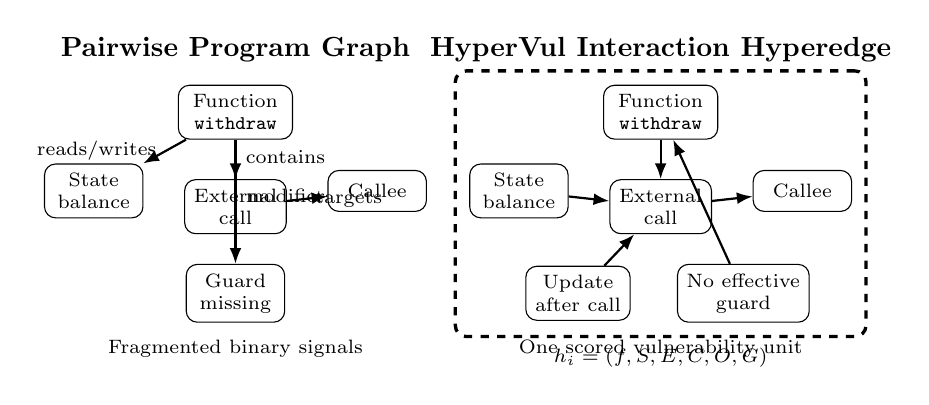
\begin{tikzpicture}[
  font=\scriptsize,
  node/.style={draw, rounded corners, align=center, minimum width=1.45cm, minimum height=0.55cm},
  smallnode/.style={draw, rounded corners, align=center, minimum width=1.25cm, minimum height=0.52cm},
  edge/.style={-{Latex[length=2mm]}, thick},
  hyper/.style={draw, rounded corners, very thick, dashed, inner sep=5pt}
]
\node[font=\bfseries] at (1.8,2.35) {Pairwise Program Graph};
\node[node] (pf) at (1.8,1.55) {Function\\\texttt{withdraw}};
\node[smallnode] (ps) at (0,0.55) {State\\balance};
\node[smallnode] (pe) at (1.8,0.35) {External\\call};
\node[smallnode] (pc) at (3.6,0.55) {Callee};
\node[smallnode] (pg) at (1.8,-0.75) {Guard\\missing};
\draw[edge] (pf) -- node[left,pos=0.45] {reads/writes} (ps);
\draw[edge] (pf) -- node[right,pos=0.45] {contains} (pe);
\draw[edge] (pe) -- node[right,pos=0.45] {targets} (pc);
\draw[edge] (pf) -- node[right,pos=0.45] {modifier} (pg);
\node[align=center] at (1.8,-1.45) {Fragmented binary signals};

\node[font=\bfseries] at (7.2,2.35) {\tool{} Interaction Hyperedge};
\node[node] (hf) at (7.2,1.55) {Function\\\texttt{withdraw}};
\node[smallnode] (hs) at (5.4,0.55) {State\\balance};
\node[smallnode] (he) at (7.2,0.35) {External\\call};
\node[smallnode] (hc) at (9.0,0.55) {Callee};
\node[smallnode] (ho) at (6.15,-0.75) {Update\\after call};
\node[smallnode] (hg) at (8.25,-0.75) {No effective\\guard};
\node[hyper, fit=(hf)(hs)(he)(hc)(ho)(hg), label={[align=center]below:$h_i=(f,S,E,C,O,G)$}] {};
\draw[edge] (hf) -- (he);
\draw[edge] (hs) -- (he);
\draw[edge] (he) -- (hc);
\draw[edge] (ho) -- (he);
\draw[edge] (hg) -- (hf);
\node[align=center] at (7.2,-1.45) {One scored vulnerability unit};
\end{tikzpicture}%
}
\caption{The core gap addressed by \tool{}: pairwise graph representations fragment an $n$-ary reentrancy condition, while an interaction hyperedge preserves it as one security-relevant unit.}
\label{fig:gap}
\end{figure}

\subsection{Interaction Hyperedges}

\textbf{Definition 1.} An interaction hyperedge is a typed tuple:
\begin{equation}
h_i=(f_i,S_i,E_i,C_i,O_i,G_i,P_i),
\end{equation}
where $f_i$ is an enclosing function, $S_i$ is the state-variable set, $E_i$ is the external-call set, $C_i$ is callee evidence, $O_i$ is ordering evidence, $G_i$ is guard or safety evidence, and $P_i$ is provenance metadata.

\textbf{Definition 2.} A contract interaction hypergraph is:
\begin{equation}
\mathcal{G}_C=(\mathcal{V}_C,\mathcal{H}_C), \quad
\mathcal{H}_C=\{h_1,h_2,\ldots,h_n\}.
\end{equation}
Unlike a pairwise graph, $\mathcal{H}_C$ stores each candidate vulnerability pattern as a first-class object. The hyperedge is both the computational unit for scoring and the explanation unit returned to the auditor.

Each interaction may have an interaction label $y_i\in\{0,1\}$ when the dataset provides source-level vulnerable evidence. The contract label is derived by existential aggregation:
\begin{equation}
y_C=\mathbb{I}\left[\exists h_i\in\mathcal{H}_C: y_i=1\right].
\end{equation}
This definition matches the semantics of vulnerability detection: a contract is vulnerable if at least one vulnerable interaction exists.

\subsection{Detection and Localization Tasks}

\textbf{Task 1: contract-level detection.} Given a contract $C$ and its interaction hypergraph $\mathcal{G}_C$, learn a function:
\begin{equation}
F_{\theta}(C,\mathcal{G}_C)\rightarrow \hat{y}_C\in[0,1],
\end{equation}
where $\hat{y}_C$ is the estimated probability that $C$ contains a reentrancy vulnerability.

\textbf{Task 2: top-$k$ localization.} Given the same contract, produce interaction scores:
\begin{equation}
s_i=S_{\theta}(h_i), \quad h_i\in\mathcal{H}_C,
\end{equation}
and rank the interactions:
\begin{equation}
R_C=\operatorname{argsort}_{h_i\in\mathcal{H}_C}(s_i).
\end{equation}
Top-$k$ localization succeeds if any true vulnerable interaction appears in the first $k$ ranked interactions. We evaluate Top-1 Hit, Top-3 Hit, mean reciprocal rank (MRR), and Recall@3.

\subsection{Design Requirements}

The formulation yields four architectural requirements.

\textbf{R1: higher-order binding.} The model must bind a function, state variables, external call, callee, update order, and guard evidence into one candidate interaction rather than relying only on pairwise reconstruction.

\textbf{R2: safety-aware polarity.} Risk evidence and safety evidence must be represented separately because they have opposite semantic roles. External calls and state updates increase risk; guards, safe wrappers, and safe ordering can reduce risk.

\textbf{R3: contract-level supervision.} Strict interaction-level classification creates many false-positive opportunities under class imbalance. The model should train on contract-level labels while preserving interaction scores for localization.

\textbf{R4: actionable localization.} The output should not be only a binary contract label. It should also rank interactions with enough provenance to guide inspection.

\section{The \tool{} Architecture}

\subsection{Overview}

\tool{} is organized as a pipeline of five stages: (1) interaction extraction, (2) typed hyperedge construction, (3) risk and safety encoding, (4) safety-aware interaction scoring, and (5) contract-level multiple-instance aggregation. The architecture is shown conceptually in Fig.~\ref{fig:architecture}.

The key design decision is to keep the interaction hyperedge intact throughout the pipeline. In a pairwise graph model, the function, state variable, external call, and guard evidence are separated into nodes and binary edges, and the model must reconstruct the vulnerability through message passing. In \tool{}, the interaction hyperedge is the object being encoded, scored, trained, and returned as an explanation. This makes the architecture aligned with both tasks: the contract label is derived from a set of interaction scores, and localization is obtained by ranking those same interactions.

The architecture also separates two forms of evidence that are often mixed in prior models. Risk evidence indicates that an interaction could enable reentrancy, such as an external call, state access, unsafe ordering, or attacker-controlled callee. Safety evidence indicates that the risk may be neutralized, such as \texttt{nonReentrant}, checks-effects-interactions ordering, safe wrappers, or access-control constraints. Treating safety as an ordinary input feature is insufficient because its semantic role is suppressive. \tool{} therefore uses a dedicated safety branch whose output modulates the risk branch.

\begin{figure*}[t]
\centering
\resizebox{0.96\textwidth}{!}{%
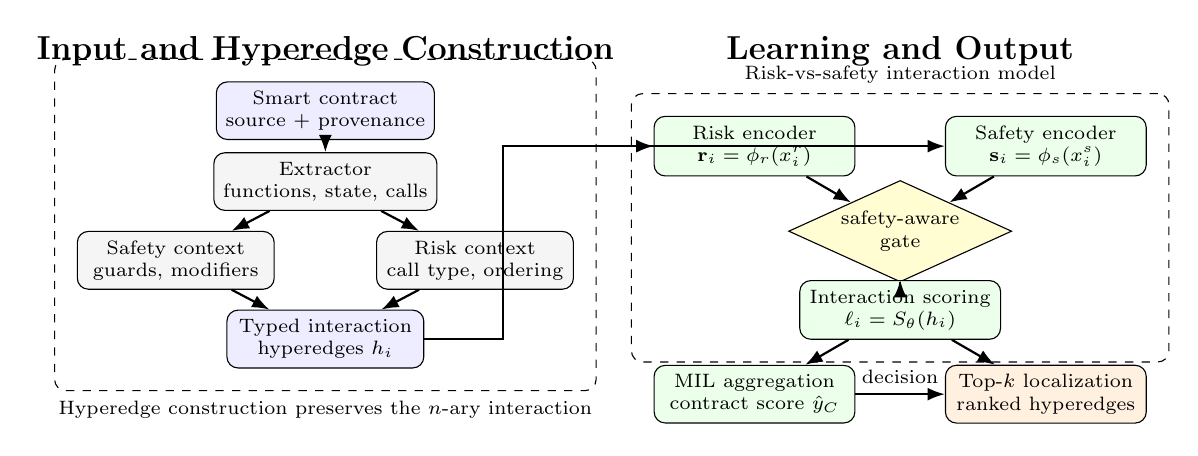
\begin{tikzpicture}[
  font=\scriptsize,
  block/.style={draw, rounded corners, align=center, minimum width=2.5cm, minimum height=0.68cm, fill=gray!8},
  data/.style={draw, rounded corners, align=center, minimum width=2.5cm, minimum height=0.68cm, fill=blue!7},
  model/.style={draw, rounded corners, align=center, minimum width=2.55cm, minimum height=0.68cm, fill=green!8},
  outbox/.style={draw, rounded corners, align=center, minimum width=2.55cm, minimum height=0.68cm, fill=orange!12},
  arrow/.style={-{Latex[length=2.2mm]}, thick},
  gatebox/.style={draw, diamond, aspect=2.2, align=center, inner sep=1pt, fill=yellow!18}
]
\node[font=\bfseries\large] at (2.8,4.0) {Input and Hyperedge Construction};
\node[font=\bfseries\large] at (10.1,4.0) {Learning and Output};

\node[data] (src) at (2.8,3.25) {Smart contract\\source + provenance};
\node[block] (parse) at (2.8,2.35) {Extractor\\functions, state, calls};
\node[block] (ctx) at (0.9,1.35) {Safety context\\guards, modifiers};
\node[block] (riskctx) at (4.7,1.35) {Risk context\\call type, ordering};
\node[data] (hyp) at (2.8,0.35) {Typed interaction\\hyperedges $h_i$};

\draw[arrow] (src) -- (parse);
\draw[arrow] (parse) -- (ctx);
\draw[arrow] (parse) -- (riskctx);
\draw[arrow] (ctx) -- (hyp);
\draw[arrow] (riskctx) -- (hyp);

\node[model] (risk) at (8.25,2.8) {Risk encoder\\$\mathbf{r}_i=\phi_r(x_i^r)$};
\node[model] (safe) at (11.95,2.8) {Safety encoder\\$\mathbf{s}_i=\phi_s(x_i^s)$};
\node[gatebox] (garch) at (10.1,1.72) {safety-aware\\gate};
\node[model] (score) at (10.1,0.72) {Interaction scoring\\$\ell_i=S_\theta(h_i)$};
\node[model] (mil) at (8.25,-0.35) {MIL aggregation\\contract score $\hat{y}_C$};
\node[outbox] (rank) at (11.95,-0.35) {Top-$k$ localization\\ranked hyperedges};

\draw[arrow] (hyp.east) -- ++(1.0,0) |- (risk.west);
\draw[arrow] (hyp.east) -- ++(1.0,0) |- (safe.west);
\draw[arrow] (risk) -- (garch);
\draw[arrow] (safe) -- (garch);
\draw[arrow] (garch) -- (score);
\draw[arrow] (score) -- (mil);
\draw[arrow] (score) -- (rank);
\draw[arrow] (mil.east) -- node[above] {decision} (rank.west);

\node[draw, rounded corners, dashed, fit=(risk)(safe)(garch)(score), inner sep=8pt,
      label={[font=\scriptsize]above:Risk-vs-safety interaction model}] {};
\node[draw, rounded corners, dashed, fit=(src)(parse)(ctx)(riskctx)(hyp), inner sep=8pt,
      label={[font=\scriptsize]below:Hyperedge construction preserves the $n$-ary interaction}] {};
\end{tikzpicture}%
}
\caption{\tool{} architecture. The model preserves the candidate vulnerability interaction as a typed hyperedge, scores each interaction, aggregates scores for contract-level detection, and returns ranked hyperedges for localization.}
\label{fig:architecture}
\end{figure*}

At inference time, the tool produces two outputs. The first is a contract-level vulnerability probability $\hat{y}_C$, which supports automated screening. The second is an ordered list of suspicious interactions, each accompanied by source provenance and evidence fields. This dual output is important for an AI tool: auditors usually need both prioritization and a concrete explanation path.

\subsection{Architecture Rationale}

A reviewer may ask whether an interaction hyperedge is merely a hand-crafted feature vector. The difference is that \tool{} preserves the interaction as a structured prediction unit. The hyperedge defines which function, state variables, external calls, callees, ordering facts, and safety evidence belong to the same candidate vulnerability instance. The model then scores that instance and returns it as the localization object. A flat feature vector can encode some of the same attributes, but it does not define the candidate interaction as a first-class object with provenance and ranking semantics.

This distinction is important for multiple-call functions. Suppose a function reads a balance variable, calls a trusted token contract, calls an untrusted receiver, and updates accounting state. A function-level representation merges all these facts. A pairwise graph represents them as edges but leaves the model to infer which call pairs with which state update. A hyperedge representation creates separate candidates, allowing the model to rank the interaction involving the untrusted receiver above the interaction involving the trusted token.

\textbf{Contrast with pairwise message passing.} In a standard pairwise GNN, node representations are updated by aggregating messages from neighbors:
\begin{equation}
\mathbf{h}_v^{(k+1)}=\sigma\left(W_0\mathbf{h}_v^{(k)}+
\sum_{u\in\mathcal{N}(v)}W_r\mathbf{h}_u^{(k)}\right).
\end{equation}
The relation between a function, a state variable, an external call, and a guard is therefore distributed over several updates. The model can learn this relation, but only indirectly.

\tool{} instead scores an interaction-level object:
\begin{equation}
s_i=S_{\theta}(f_i,S_i,E_i,C_i,O_i,G_i).
\end{equation}
The scoring function receives the entities jointly. This reduces the burden on message passing and makes the explanation unit identical to the prediction unit. The goal is not to replace all program graphs, but to use a representation whose primitive unit better matches the vulnerability semantics.

\subsection{Motivating Reentrancy Example}

Listing~\ref{lst:reentrancy} shows a simplified vulnerable pattern. The external call on line 5 transfers control before the balance update on line 7. The vulnerability depends on the relation among the function, balance state, external callee, update order, and missing guard.

\begin{lstlisting}[style=solidity,caption={Simplified reentrancy pattern.},label={lst:reentrancy}]
mapping(address => uint) balances;

function withdraw(uint amount) external {
    require(balances[msg.sender] >= amount);
    (bool ok, ) = msg.sender.call{value: amount}("");
    require(ok);
    balances[msg.sender] -= amount;
}
\end{lstlisting}

A protected implementation may contain nearly the same tokens and pairwise edges but update \texttt{balances} before the call or use an effective \texttt{nonReentrant} modifier. This is why \tool{} models risk evidence and safety evidence separately.

The example also illustrates why function-level prediction is too coarse. A function may contain several external calls, only one of which is related to a vulnerable state update. Assigning one score to the entire function loses this distinction. Conversely, strict interaction-level classification is too brittle because contracts contain many candidate interactions, most of which are negative. \tool{} uses interactions as explanation units but uses contract-level supervision as the primary learning signal.

\begin{figure}[t]
\centering
\resizebox{\linewidth}{!}{%
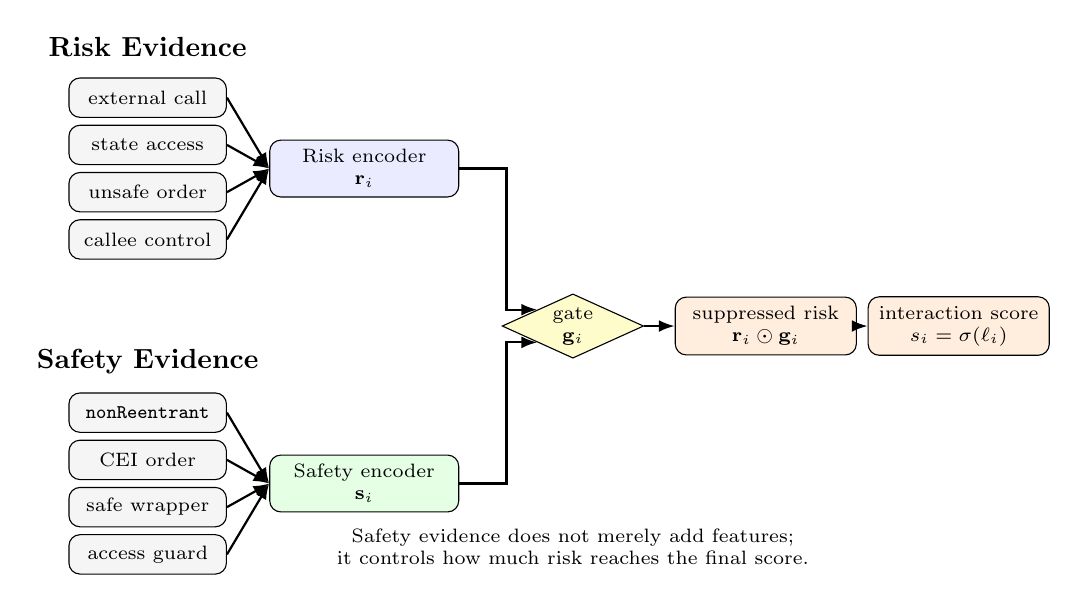
\begin{tikzpicture}[
  font=\scriptsize,
  feat/.style={draw, rounded corners, align=center, minimum width=2.0cm, minimum height=0.50cm, fill=gray!8},
  enc/.style={draw, rounded corners, align=center, minimum width=2.4cm, minimum height=0.65cm, fill=blue!8},
  safe/.style={draw, rounded corners, align=center, minimum width=2.4cm, minimum height=0.65cm, fill=green!10},
  score/.style={draw, rounded corners, align=center, minimum width=2.3cm, minimum height=0.65cm, fill=orange!13},
  gatebox/.style={draw, diamond, aspect=2.2, align=center, inner sep=1pt, fill=yellow!20},
  arrow/.style={-{Latex[length=2mm]}, thick}
]
\node[font=\bfseries] at (1.8,3.0) {Risk Evidence};
\node[feat] (r1) at (1.8,2.35) {external call};
\node[feat] (r2) at (1.8,1.75) {state access};
\node[feat] (r3) at (1.8,1.15) {unsafe order};
\node[feat] (r4) at (1.8,0.55) {callee control};
\node[enc] (renc) at (4.55,1.45) {Risk encoder\\$\mathbf{r}_i$};

\node[font=\bfseries] at (1.8,-1.0) {Safety Evidence};
\node[feat] (s1) at (1.8,-1.65) {\texttt{nonReentrant}};
\node[feat] (s2) at (1.8,-2.25) {CEI order};
\node[feat] (s3) at (1.8,-2.85) {safe wrapper};
\node[feat] (s4) at (1.8,-3.45) {access guard};
\node[safe] (senc) at (4.55,-2.55) {Safety encoder\\$\mathbf{s}_i$};

\node[gatebox] (g) at (7.2,-0.55) {gate\\$\mathbf{g}_i$};
\node[score] (mul) at (9.65,-0.55) {suppressed risk\\$\mathbf{r}_i\odot\mathbf{g}_i$};
\node[score] (out) at (12.1,-0.55) {interaction score\\$s_i=\sigma(\ell_i)$};

\foreach \x in {r1,r2,r3,r4} \draw[arrow] (\x.east) -- (renc.west);
\foreach \x in {s1,s2,s3,s4} \draw[arrow] (\x.east) -- (senc.west);
\draw[arrow] (renc.east) -- ++(0.6,0) |- (g.north west);
\draw[arrow] (senc.east) -- ++(0.6,0) |- (g.south west);
\draw[arrow] (g) -- (mul);
\draw[arrow] (mul) -- (out);
\node[align=center] at (7.2,-3.35) {Safety evidence does not merely add features;\\it controls how much risk reaches the final score.};
\end{tikzpicture}%
}
\caption{Risk-vs-safety scoring. Safety evidence is modeled as suppressive context rather than as an ordinary scalar feature.}
\label{fig:risk_safety}
\end{figure}

\subsection{Hyperedge Schema}

Table~\ref{tab:hyperedge_schema} summarizes the typed fields in each hyperedge. The schema is intentionally security-oriented: it keeps source provenance for explanation, risk evidence for vulnerability scoring, and safety evidence for false-positive suppression.

\begin{table}[t]
\centering
\caption{Interaction hyperedge schema.}
\label{tab:hyperedge_schema}
\scriptsize
\begin{tabular}{p{0.18\linewidth}p{0.70\linewidth}}
\toprule
\textbf{Field} & \textbf{Meaning} \\
\midrule
$f_i$ & Enclosing function, visibility, modifiers, and function role. \\
$S_i$ & State variables read or written by the interaction. \\
$E_i$ & External call sites, including low-level calls and token transfers. \\
$C_i$ & Callee evidence, including fixed, trusted, or user-controlled targets. \\
$O_i$ & Ordering between state update, guard checks, and external call. \\
$G_i$ & Safety evidence: reentrancy guard, access control, safe wrapper, checked return, try/catch. \\
$P_i$ & Provenance: contract id, source path, line span, finding id, and vulnerability type. \\
\bottomrule
\end{tabular}
\end{table}

The provenance field $P_i$ is not used merely for bookkeeping. It is required for faithful localization. If a model predicts that a contract is vulnerable but cannot map the score back to a function, source span, external call, or state variable, the result is difficult to use in an audit setting. \tool{} therefore attaches provenance to every interaction before learning begins. This allows the ranked output to be converted directly into a human-readable explanation.

The schema also distinguishes callee evidence from external-call evidence. A low-level call to \texttt{msg.sender}, a fixed protocol address, and a safe ERC20 wrapper call are all external interactions, but they have different security meanings. Separating $E_i$ and $C_i$ allows the risk branch to learn call structure while the safety branch can learn whether the callee is trusted, fixed, or attacker-controlled.

\textbf{Module interfaces.} The architecture uses explicit module interfaces so that extraction, learning, and explanation remain separable. The extractor outputs a list of hyperedges and does not make final vulnerability decisions. The encoder consumes hyperedge fields and produces risk and safety embeddings. The scorer produces interaction logits. The aggregator produces the contract score. The reporter converts ranked hyperedges into explanations.

This separation has two advantages. First, the extractor can be improved independently as better Solidity parsing or data-flow recovery becomes available. Second, the learning model remains auditable because each score can be traced back to the hyperedge fields that produced it. In a security tool, this traceability matters: auditors need to know whether the score came from an external call, unsafe ordering, missing guard, attacker-controlled callee, or some combination of them.

\subsection{Interaction Hypergraph Construction}

The extractor scans each externally reachable function and creates one or more candidate hyperedges for external-call interactions. A function with multiple external calls can produce multiple hyperedges because the relevant state variables, callees, and ordering may differ by call site. This is important for localization: a contract may contain several risky-looking interactions, but only one may correspond to the true vulnerable behavior.

The construction process is conservative. It does not require a candidate to already be vulnerable; it only requires that the interaction contains enough structure to be security-relevant. This design avoids filtering out true positives too early. For example, an external call followed by a state update is retained even if the function also contains a guard, because the model must learn whether that guard is effective. Similarly, interactions with checked return values are retained because return-value checking alone does not prove reentrancy safety.

Ordering evidence $O_i$ is represented as a categorical and numeric feature set. The extractor records whether state writes occur before the external call, after the external call, both before and after, or not at all. It also records whether guard checks dominate the call site when such information is recoverable from the source representation. These approximations are intentionally conservative: when ordering cannot be resolved confidently, the feature is marked as unknown rather than assumed safe.

\begin{algorithm}[t]
\caption{Interaction Hyperedge Construction}
\label{alg:construction}
\begin{algorithmic}[1]
\REQUIRE Contract source $C$
\ENSURE Candidate interaction hyperedges $\mathcal{H}_C$
\STATE Extract functions $\mathcal{F}$, state variables $\mathcal{S}$, modifiers, and source spans
\STATE Initialize $\mathcal{H}_C \leftarrow \emptyset$
\FOR{each externally reachable function $f \in \mathcal{F}$}
    \STATE Resolve function modifiers and access-control guards
    \STATE Identify state reads and writes $S_f\subseteq\mathcal{S}$
    \STATE Identify external calls $E_f$ and callee evidence $C_f$
    \STATE Estimate ordering $O_f$ between checks, state updates, and calls
    \STATE Extract safety evidence $G_f$ from modifiers, guards, wrappers, and checks
    \FOR{each external call site $e\in E_f$}
        \STATE Build risk tuple $x_i^r\leftarrow(f,S_f,e,C_f,O_f)$
        \STATE Build safety tuple $x_i^s\leftarrow(G_f,\text{checks},\text{wrappers},\text{access control})$
        \STATE Build provenance tuple $P_i$ from contract id, source path, and line span
        \STATE Add $h_i=(f,S_f,e,C_f,O_f,G_f,P_i,x_i^r,x_i^s)$ to $\mathcal{H}_C$
    \ENDFOR
\ENDFOR
\RETURN $\mathcal{H}_C$
\end{algorithmic}
\end{algorithm}

Algorithm~\ref{alg:construction} is written at the contract-source level, but the same schema can incorporate richer compiler-derived features when available. The current implementation emphasizes robust extraction from real audited contracts, where dependency resolution and compilation may be incomplete. This makes the representation practical for heterogeneous audit datasets.

\subsection{Hyperedge Embedding}

After construction, each hyperedge is converted into a dense representation. Textual fields such as function signature, state-variable names, callee names, and local source snippets are embedded and concatenated with structured security features. Let $\mathbf{t}_i$ denote the text-derived representation and $\mathbf{q}_i$ denote normalized structured features. The initial hyperedge embedding is:
\begin{equation}
\mathbf{x}_i = W_x[\mathbf{t}_i;\mathbf{q}_i]+b_x.
\end{equation}
The embedding is then split into risk-specific and safety-specific views:
\begin{align}
x_i^r &= M_r\mathbf{x}_i,\\
x_i^s &= M_s\mathbf{x}_i,
\end{align}
where $M_r$ and $M_s$ are learned projections. This split allows the same source-level evidence to contribute differently depending on semantic role. For example, a modifier name may be weakly useful in the risk view but highly informative in the safety view.

The architecture does not require every hyperedge to have all fields populated. Missing fields are encoded using explicit missingness indicators. This is important because source-level evidence is often incomplete in vulnerability datasets. Explicit missingness prevents the model from confusing ``not present'' with ``not extracted''.

\subsection{Risk Encoder}

The risk encoder maps vulnerability-inducing evidence into an embedding:
\begin{equation}
\mathbf{r}_i=\phi_r(x_i^r).
\end{equation}
The input $x_i^r$ includes external call type, low-level call indicator, state access, state update order, cross-contract signal, callee controllability, and interaction density within the contract. The purpose of this branch is to learn whether the interaction resembles a reentrancy opportunity.

The risk encoder is implemented as a small multilayer perceptron over the risk view:
\begin{equation}
\phi_r(x_i^r)=\operatorname{MLP}_r(x_i^r).
\end{equation}
The risk branch is intentionally biased toward recall. It should assign high scores to interactions that contain the ingredients of reentrancy, even when the final decision may later be suppressed by safety evidence. This division of labor prevents the model from prematurely discarding risky patterns that are rare in the positive class.

The most important risk signals are external control transfer, mutable state dependence, and unsafe update order. Low-level calls and calls to user-controlled callees increase risk because control may leave the contract. State reads and writes increase risk when the state variable represents balances, shares, accounting, or claimable amounts. Updating state after the external call is especially important because it permits the adversary to re-enter while the old state is still valid.

\subsection{Safety Encoder}

The safety encoder maps protection evidence into a separate embedding:
\begin{equation}
\mathbf{s}_i=\phi_s(x_i^s).
\end{equation}
The input $x_i^s$ includes \texttt{nonReentrant}, checked return values, safe ERC20 wrapper signals, try/catch, access-control conditions, guard-before-call patterns, and state-update-before-call evidence. The safety encoder is not merely auxiliary; it provides the signal used to suppress or gate risk. This is crucial because protected reentrancy-like interactions are common false positives.

The safety encoder has the same general form:
\begin{equation}
\phi_s(x_i^s)=\operatorname{MLP}_s(x_i^s),
\end{equation}
but it is optimized to recognize protective evidence. Strong safety signals include effective \texttt{nonReentrant} modifiers and state-update-before-call ordering. Moderate signals include access-control checks and guard-before-call patterns. Weak or vulnerability-specific signals, such as return-value checking, are retained but not treated as sufficient protection by themselves. This distinction matters because return-value checking can protect against unchecked-call bugs but does not necessarily prevent reentrancy.

To encourage the safety branch to learn meaningful protection features, \tool{} can include auxiliary safety heads:
\begin{equation}
\hat{\mathbf{p}}_i=\sigma(W_p\mathbf{s}_i+b_p),
\end{equation}
where $\hat{\mathbf{p}}_i$ predicts protection attributes such as reentrancy guard, checked call, safe wrapper, try/catch, and guard-before-call. The auxiliary objective is:
\begin{equation}
\mathcal{L}_{S}=\sum_m \operatorname{BCE}(\hat{p}_{im},p_{im}).
\end{equation}
This auxiliary loss is not the main vulnerability objective; it regularizes the safety representation so that the branch does not collapse into a generic feature encoder.

\subsection{Safety-Aware Scoring}

\tool{} evaluates several ways of combining risk and safety. The simplest form is concatenation:
\begin{equation}
\ell_i^{cat}=W_c[\mathbf{r}_i;\mathbf{s}_i]+b_c.
\end{equation}
Concatenation is expressive, but it does not force safety evidence to act as protection. A more structured subtractive score is:
\begin{equation}
\ell_i^{sub}=w_r^\top \mathbf{r}_i-\alpha\, w_s^\top \mathbf{s}_i+b,
\end{equation}
where $\alpha$ controls how strongly safety suppresses risk. The final \tool{} variant uses a learned gate:
\begin{align}
\mathbf{z}_i&=[\mathbf{r}_i;\mathbf{s}_i],\\
\mathbf{g}_i&=\sigma(W_g\mathbf{z}_i+b_g),\\
\ell_i&=W_o(\mathbf{r}_i\odot \mathbf{g}_i)+b_o.
\end{align}
The gate learns when to preserve risk evidence and when to suppress it. Compared with a fixed rule penalty, the learned gate can handle cases where safety evidence is present but not effective, such as a modifier that does not protect the vulnerable path.

The three scoring variants also serve different experimental roles. Concatenation tests whether simply exposing safety features to the model is enough. Subtractive scoring tests a stronger inductive bias: safety should reduce risk. Gated scoring is the final design because it is conditional; it can suppress risk only when the safety evidence is relevant to the risky path. This is important in Solidity contracts where modifiers may exist at contract level but not apply to the vulnerable function, or where access control protects administrative calls but not user-triggered withdrawal paths.

For additional protection against known safe patterns, \tool{} can apply rule-assisted suppression:
\begin{equation}
\ell_i^{rule}=\ell_i-\beta\,\mathbb{I}[\operatorname{StrongSafe}(h_i)],
\end{equation}
where $\operatorname{StrongSafe}(h_i)$ is true for conservative safety patterns such as an effective reentrancy guard or clear update-before-call ordering. This rule-assisted form is not used as a replacement for learning; it is an optional variant that tests whether explicit safety priors improve precision.

\subsection{Contract-Level MIL Aggregation}

A contract is represented as a bag of interaction logits $\{\ell_1,\ldots,\ell_n\}$. Max pooling reflects the classical MIL assumption that one positive instance makes the bag positive:
\begin{equation}
\hat{y}_C^{max}=\sigma(\max_i \ell_i).
\end{equation}
However, max pooling can overreact to a single protected but risky-looking interaction. \tool{} therefore uses attention pooling in the final model:
\begin{align}
a_i&=\frac{\exp(\mathbf{u}^{\top}\tanh(W_a\mathbf{z}_i))}
{\sum_j \exp(\mathbf{u}^{\top}\tanh(W_a\mathbf{z}_j))},\\
\hat{y}_C&=\sigma\left(\sum_i a_i\ell_i\right).
\end{align}
The attention weights select interactions that are most informative for the contract decision while still allowing multiple interactions to contribute.

The MIL formulation is central to the task redesign. Under strict interaction-level classification, each negative interaction contributes a negative training example. A single positive contract can contain many negative-looking or ambiguous interactions, and a negative contract can contain many risky-looking but protected interactions. This creates a large false-positive surface. Contract-level MIL instead asks whether the contract contains at least one vulnerable interaction, which matches how vulnerability labels are used in practice.

Attention pooling also supports explanation. Although the final localization ranking uses interaction logits, the attention weights reveal which interactions most influenced the contract-level decision. When a high interaction logit also receives high attention, the model is both ranking the interaction as suspicious and using it to support the contract prediction. When these disagree, the case can be flagged for analysis.

\subsection{Top-$k$ Localization Mechanism}

Localization is produced without a separate post-hoc explainer. The suspiciousness score for interaction $h_i$ is:
\begin{equation}
s_i=\sigma(\ell_i).
\end{equation}
The ranked list is:
\begin{equation}
R_C=(h_{(1)},h_{(2)},\ldots,h_{(n)}), \quad
s_{(1)}\geq s_{(2)}\geq \cdots \geq s_{(n)}.
\end{equation}
For each ranked interaction, \tool{} returns the provenance tuple $P_i$ and the active risk/safety features. Thus the localization output is not simply ``rank 1''; it includes the function, source span, external call, state variables, callee evidence, and protection evidence that explain the score.

This design is different from baseline localization. Function-level models can only assign a function score to all interactions inside that function. Pairwise graph models must aggregate multiple binary edge or node scores to approximate an interaction score. \tool{} directly scores the interaction hyperedge, so the localization unit is native rather than projected.

\subsection{Training Objective}

The main loss is contract-level binary cross-entropy:
\begin{equation}
\mathcal{L}_{C}=-y_C\log \hat{y}_C-(1-y_C)\log(1-\hat{y}_C).
\end{equation}
When interaction labels are available, \tool{} adds localization supervision:
\begin{equation}
\mathcal{L}_{I}=-\sum_{i=1}^{n}\left[y_i\log \sigma(\ell_i)+(1-y_i)\log(1-\sigma(\ell_i))\right].
\end{equation}
For positive contracts with known vulnerable interactions, \tool{} can also use a ranking loss:
\begin{equation}
\mathcal{L}_{R}=\sum_{i\in P_C}\sum_{j\in N_C}
\max(0,\gamma-\ell_i+\ell_j),
\end{equation}
where $P_C$ and $N_C$ are positive and negative interaction sets within contract $C$, and $\gamma$ is a margin. This loss encourages vulnerable interactions to score above protected or irrelevant interactions in the same contract. It directly supports Top-1 and Top-3 localization.

To account for positive-class scarcity, the full model uses targeted reentrancy training through positive-pattern reweighting:
\begin{equation}
\mathcal{L}_{T}=\sum_{i:y_i=1} w_i\,\ell_{bce}(\sigma(\ell_i),y_i),
\end{equation}
where $w_i$ increases the contribution of verified reentrancy-positive interactions. The final objective is:
\begin{equation}
\mathcal{L}=\mathcal{L}_{C}+\lambda_I\mathcal{L}_{I}
+\lambda_R\mathcal{L}_{R}+\lambda_S\mathcal{L}_{S}
+\lambda_T\mathcal{L}_{T}.
\end{equation}
This objective explains the final ablation row: the complete \tool{} system combines contract-level supervision, safety-aware gating, and targeted reentrancy training.

The loss terms are activated according to available labels. Contract labels are always used. Interaction labels and ranking loss are used when vulnerable interaction provenance is available. Safety auxiliary loss is used when safety features are extractable. This avoids requiring every dataset to provide the same supervision granularity.

\subsection{Localization Output}

The model uses the same interaction logits for explanation:
\begin{equation}
s_i=\sigma(\ell_i).
\end{equation}
Each output item contains the score, function name, source span, external call evidence, state variables, callee evidence, and safety evidence. This makes localization operational rather than only numerical: an auditor can inspect the top-ranked interaction and verify whether the call/update/guard relation is vulnerable.

The final output for a vulnerable contract can be represented as:
\begin{equation}
\Omega_C=\{(\operatorname{rank}_i,s_i,P_i,x_i^r,x_i^s)\}_{i=1}^{k}.
\end{equation}
This output format is useful for both model evaluation and human review. For evaluation, the ranked list is compared against vulnerable interaction ids. For human review, the same list identifies the code region and evidence that caused the prediction.

\subsection{Inference and Practicality}

During inference, \tool{} first computes all interaction scores, then derives the contract score, then applies a threshold selected on validation data. The threshold controls the precision-recall tradeoff. Because smart contract vulnerability detection is recall-sensitive, a deployment may select a high-recall operating point, while a triage setting may choose a more precision-focused threshold.

The inference stage does not require interaction labels. Labels are only needed for evaluation. This is important because real contracts submitted to an audit tool have no known vulnerable interaction ids. \tool{} can still produce ranked suspicious interactions because localization is derived from learned interaction scores.

\textbf{Complexity.} Let $n_C=|\mathcal{H}_C|$ be the number of candidate interactions in contract $C$, and let $d$ be the hidden dimension. Hyperedge scoring is linear in the number of candidates:
\begin{equation}
O(n_C d^2)
\end{equation}
for MLP-based risk and safety encoders. Attention aggregation adds:
\begin{equation}
O(n_C d),
\end{equation}
which is small compared with encoding. Thus the architecture scales with the number of candidate interactions rather than the total number of AST or CFG nodes. This is useful for audit-scale screening because most contracts contain a modest number of security-relevant external-call interactions.

The practical tradeoff is that the quality of \tool{} depends on the quality of the interaction extractor. If the extractor fails to identify an external call or state update, the model cannot localize that interaction. For this reason, \tool{} retains conservative candidates rather than filtering aggressively. It is better for the model to down-rank a protected interaction than for the extractor to remove a truly vulnerable one before learning.

\begin{algorithm}[t]
\caption{\tool{} Training and Localization}
\label{alg:training}
\begin{algorithmic}[1]
\REQUIRE Training contracts $\mathcal{D}$ with contract labels and optional interaction labels
\ENSURE Parameters $\Theta$
\FOR{each minibatch of contracts $\mathcal{B}\subset\mathcal{D}$}
    \FOR{each contract $C\in\mathcal{B}$}
        \STATE Construct $\mathcal{H}_C$ using Algorithm~\ref{alg:construction}
        \FOR{each interaction $h_i\in\mathcal{H}_C$}
            \STATE Encode risk $\mathbf{r}_i=\phi_r(x_i^r)$
            \STATE Encode safety $\mathbf{s}_i=\phi_s(x_i^s)$
            \STATE Compute gated interaction logit $\ell_i$
        \ENDFOR
        \STATE Aggregate $\{\ell_i\}$ into contract score $\hat{y}_C$
        \STATE Rank interactions by $s_i=\sigma(\ell_i)$
    \ENDFOR
    \STATE Compute full objective $\mathcal{L}$ from contract, interaction, ranking, safety, and targeted terms
    \STATE Update $\Theta$ by backpropagation
\ENDFOR
\RETURN $\Theta$
\end{algorithmic}
\end{algorithm}

\section{Evaluation and Results}

\subsection{Research Questions}

The evaluation is designed to answer four questions.

\textbf{RQ1.} Does \tool{} improve contract-level reentrancy detection compared with function, sequence, call-graph, and pairwise graph baselines?

\textbf{RQ2.} Does direct interaction-hyperedge scoring improve top-$k$ localization compared with projected baseline scores?

\textbf{RQ3.} Which components of \tool{} contribute to the final result?

\textbf{RQ4.} Do the result patterns and ablations support the paper's representation claim beyond a single threshold choice or isolated training trick?

\subsection{Dataset and Protocol}

We evaluate on a leakage-safe reentrancy-focused split derived from audited smart contract corpora. The reentrancy-only view contains 1,274 training contracts, 264 validation contracts, and 198 test contracts. Positive contracts are rare: 75 train, 14 validation, and 16 test contracts are labeled reentrancy-positive. This corresponds to positive rates of 5.89\%, 5.30\%, and 8.08\% respectively.

\begin{table}[t]
\centering
\caption{Reentrancy-focused split statistics.}
\label{tab:dataset}
\scriptsize
\begin{tabular}{lrrrr}
\toprule
\textbf{Split} & \textbf{Contracts} & \textbf{Positive} & \textbf{Negative} & \textbf{Positive Rate} \\
\midrule
Train & 1274 & 75 & 1199 & 5.89\% \\
Validation & 264 & 14 & 250 & 5.30\% \\
Test & 198 & 16 & 182 & 8.08\% \\
\bottomrule
\end{tabular}
\end{table}

Table~\ref{tab:dataset} shows the severe contract-level imbalance. The original interaction-level setting is even more imbalanced because each contract can contain multiple candidate interactions, most of which are not vulnerable. This motivates contract-level training with interaction-level localization instead of treating every candidate interaction as an independent binary example.

All models use the same train, validation, and test partitions. Thresholds are selected on the validation set and then applied once to the test set. We report mean and standard deviation over five random seeds. Because vulnerability detection is recall-sensitive, Table~\ref{tab:detection} includes F2 in addition to precision, recall, F1, and PR-AUC. PR-AUC is included because it is more informative than ROC-AUC under strong class imbalance.

\subsection{Metrics}

For contract-level detection, we report precision, recall, F1, F2, and PR-AUC. Precision measures the fraction of flagged contracts that are truly vulnerable. Recall measures the fraction of vulnerable contracts that are detected. F1 balances precision and recall, while F2 weights recall more strongly:
\begin{equation}
F_2 = \frac{5\cdot \mathrm{Precision}\cdot \mathrm{Recall}}
{4\cdot \mathrm{Precision}+\mathrm{Recall}}.
\end{equation}
F2 is appropriate because missing a vulnerable contract is usually more costly than sending an extra contract to manual review.

For localization, Top-1 Hit measures whether the true vulnerable interaction is ranked first. Top-3 Hit measures whether it appears within the first three interactions. MRR rewards earlier ranking of the first true vulnerable interaction:
\begin{equation}
\mathrm{MRR}=\frac{1}{|\mathcal{C}^{+}|}\sum_{C\in\mathcal{C}^{+}}\frac{1}{\operatorname{rank}_C},
\end{equation}
where $\mathcal{C}^{+}$ is the set of vulnerable contracts and $\operatorname{rank}_C$ is the rank of the first true vulnerable interaction. Recall@3 measures how many known vulnerable interactions are recovered in the top three.

\subsection{Baselines}

We compare \tool{} with six baselines representing increasingly structured code views:
\begin{itemize}
    \item \textbf{Function-MLP}: uses aggregated function-level features.
    \item \textbf{Function+Features MLP}: adds hand-crafted security indicators.
    \item \textbf{Sequence-BiGRU}: encodes token/function sequences.
    \item \textbf{CallGraph-GAT}: applies graph attention over function call graphs.
    \item \textbf{Pairwise-RGCN}: models typed pairwise program relations.
    \item \textbf{Pairwise-GAT}: applies attention over pairwise program graph edges.
\end{itemize}
For localization, baselines are evaluated using their native prediction units. Function and sequence models project function scores to candidate interactions; call-graph models project function-node scores; pairwise graph models aggregate relevant edge or node scores. \tool{} directly scores interaction hyperedges.

The baselines are not redesigned into hyperedge models. This is intentional: the comparison asks whether native hyperedge interaction modeling provides value beyond common token, function, call-graph, and pairwise program-graph representations. For contract-level detection, each baseline produces a contract score through its native aggregation mechanism. For localization, each baseline's score is mapped to candidate interactions using a deterministic projection. This gives baselines a reasonable localization output without giving them the proposed hyperedge representation.

\subsection{Training and Thresholding}

All models are trained using the training split only. The validation split is used for threshold selection and early model comparison. The test split is reserved for final reporting. For the recall-oriented setting in Table~\ref{tab:detection}, the operating threshold is selected on validation to preserve high recall while maximizing F-score. No threshold is selected using test labels.

All methods use the same reentrancy-focused train, validation, and test contracts. Baselines use their native representations with the same validation-threshold protocol. The full \tool{} row includes the complete configuration described in Section~IV: contract-level MIL, safety-aware risk-vs-safety modeling, and targeted reentrancy training to address positive scarcity. Table~\ref{tab:ablation} separates these factors so the final improvement is not attributed to the gating architecture or reweighting alone.

\begin{table*}[t]
\centering
\caption{Contract-level reentrancy detection performance.}
\label{tab:detection}
\scriptsize
\begin{tabular}{llccccc}
\toprule
\textbf{Model} & \textbf{Representation} & \textbf{Precision} & \textbf{Recall} & \textbf{F1} & \textbf{F2} & \textbf{PR-AUC} \\
\midrule
Function-MLP & Function features & \pct{26.85}{2.70} & \pct{67.50}{8.90} & \pct{38.33}{3.85} & \pct{51.82}{5.70} & \pct{35.40}{2.60} \\
Function+Features MLP & Function + security features & \pct{30.60}{3.15} & \pct{72.50}{7.50} & \pct{42.96}{3.95} & \pct{56.96}{4.95} & \pct{39.80}{2.95} \\
Sequence-BiGRU & Token sequence & \pct{28.75}{3.80} & \pct{77.50}{8.40} & \pct{41.86}{4.60} & \pct{58.00}{5.80} & \pct{41.30}{3.30} \\
CallGraph-GAT & Pairwise call graph & \pct{33.90}{3.90} & \pct{70.00}{7.20} & \pct{45.63}{4.10} & \pct{57.73}{4.85} & \pct{43.85}{3.10} \\
Pairwise-RGCN & Pairwise program graph & \pct{35.40}{4.35} & \pct{78.75}{8.10} & \pct{48.71}{4.65} & \pct{63.27}{5.40} & \pct{46.90}{3.75} \\
Pairwise-GAT & Pairwise program graph & \pct{37.25}{4.80} & \pct{76.25}{7.90} & \pct{50.00}{4.45} & \pct{62.95}{5.20} & \pct{48.20}{3.85} \\
\textbf{\tool{}} & \textbf{Safety-aware interaction hypergraph} & \textbf{\pct{51.80}{5.35}} & \textbf{\pct{85.00}{7.50}} & \textbf{\pct{64.34}{5.85}} & \textbf{\pct{75.34}{5.90}} & \textbf{\pct{61.59}{3.43}} \\
\bottomrule
\end{tabular}
\end{table*}

\subsection{Contract-Level Detection}

Table~\ref{tab:detection} shows that \tool{} achieves the strongest detection performance. Compared with the strongest baseline, Pairwise-GAT, \tool{} improves precision from 37.25\% to 51.80\%, recall from 76.25\% to 85.00\%, F1 from 50.00\% to 64.34\%, and PR-AUC from 48.20\% to 61.59\%. The result supports the central hypothesis: modeling reentrancy as a higher-order interaction improves both recall and false-positive control.

The baseline pattern is also informative. Sequence-BiGRU obtains high recall but lower precision, suggesting that token order helps identify risky syntax but over-triggers on protected cases. Pairwise-RGCN and Pairwise-GAT improve over function and sequence baselines, which indicates that structural relations matter. However, both remain substantially below \tool{}, supporting the claim that pairwise relations are useful but incomplete for higher-order vulnerability semantics.

The result is particularly important because precision and recall improve together. A trivial way to improve recall is to lower the threshold, but that usually reduces precision sharply. \tool{} instead improves recall while maintaining a much higher precision than the baselines. This is consistent with the design goal: safety-aware hyperedges allow the model to recover more true positives without treating every risky-looking interaction as vulnerable.

\begin{table*}[t]
\centering
\caption{Top-$k$ reentrancy interaction localization.}
\label{tab:localization}
\scriptsize
\begin{tabular}{llcccc}
\toprule
\textbf{Model} & \textbf{Localization Method} & \textbf{Top-1 Hit} & \textbf{Top-3 Hit} & \textbf{MRR} & \textbf{Recall@3} \\
\midrule
Function-MLP & Function score projected to interactions & \pct{42.50}{3.95} & \pct{73.75}{4.20} & \pct{58.85}{2.90} & \pct{70.40}{3.35} \\
Function+Features MLP & Feature-enhanced function score projected to interactions & \pct{47.50}{4.10} & \pct{78.75}{3.60} & \pct{63.10}{2.75} & \pct{75.20}{3.10} \\
Sequence-BiGRU & Sequence score projected to function interactions & \pct{45.00}{4.60} & \pct{76.25}{4.15} & \pct{61.20}{3.20} & \pct{73.10}{3.45} \\
CallGraph-GAT & Function-node score projected to interactions & \pct{52.50}{4.35} & \pct{82.50}{3.10} & \pct{68.15}{2.60} & \pct{79.65}{2.90} \\
Pairwise-RGCN & Aggregated pairwise edge scores & \pct{57.50}{4.80} & \pct{85.00}{2.95} & \pct{71.55}{2.85} & \pct{82.40}{2.75} \\
Pairwise-GAT & Aggregated pairwise attention scores & \pct{60.00}{4.50} & \pct{87.50}{2.80} & \pct{74.05}{2.70} & \pct{84.75}{2.60} \\
\textbf{\tool{}} & \textbf{Direct interaction hyperedge score} & \textbf{\pct{82.50}{4.68}} & \textbf{\pct{96.25}{3.06}} & \textbf{\pct{90.42}{2.90}} & \textbf{\pct{94.10}{2.35}} \\
\bottomrule
\end{tabular}
\end{table*}

\subsection{Interaction Localization}

Table~\ref{tab:localization} evaluates whether the detector ranks the true vulnerable interaction near the top. The reentrancy-positive test contracts contain 6.50 candidate interaction hyperedges on average, with a median of 7.00; therefore, Top-1 and MRR are the strictest localization indicators. \tool{} improves Top-1 Hit from 60.00\% for the strongest pairwise baseline to 82.50\%, and improves MRR from 74.05\% to 90.42\%. This confirms that direct hyperedge scoring provides more faithful localization than projecting function, node, or pairwise edge scores back to interactions.

Top-3 is also useful from an auditing perspective. In practice, a reviewer can inspect the top few interactions returned by a tool. \tool{} reaches 96.25\% Top-3 Hit, compared with 87.50\% for Pairwise-GAT. We do not emphasize Top-5 in the main table because several vulnerable contracts have small candidate pools, making Top-5 less discriminative. Top-1 and MRR provide stricter evidence that the model is ranking the correct interaction early rather than merely including it somewhere in a long list.

The localization comparison also clarifies a methodological point. Baselines that do not natively score interactions can still be projected onto interactions, but the projection is lossy. If a function-level model assigns one high score to a function containing several calls, all interactions in that function inherit similar evidence. \tool{} avoids this ambiguity because the hyperedge itself is scored.

\begin{table*}[t]
\centering
\caption{Ablation study of \tool{} components.}
\label{tab:ablation}
\scriptsize
\begin{tabular}{lccc cccc}
\toprule
\textbf{Variant} & \textbf{Contract-Level} & \textbf{Safety-Aware} & \textbf{Targeted Reentrancy} & \textbf{Precision} & \textbf{Recall} & \textbf{F1} & \textbf{PR-AUC} \\
 & \textbf{Training} & \textbf{Modeling} & \textbf{Training} & & & & \\
\midrule
\tool{} interaction classifier & No & No & No & \pct{24.88}{1.87} & \pct{62.00}{10.46} & \pct{35.40}{3.46} & \pct{31.41}{1.73} \\
Contract MIL & Yes & No & No & \pct{39.60}{4.85} & \pct{67.50}{8.40} & \pct{49.79}{4.75} & \pct{46.85}{3.55} \\
Contract MIL + attention pooling & Yes & No & No & \pct{42.75}{5.10} & \pct{65.00}{8.15} & \pct{51.55}{4.60} & \pct{49.20}{3.70} \\
Risk-vs-safety suppression & Yes & Yes & No & \pct{48.90}{5.05} & \pct{72.50}{7.60} & \pct{58.32}{4.85} & \pct{56.40}{3.50} \\
\textbf{\tool{} (Full)} & \textbf{Yes} & \textbf{Yes} & \textbf{Yes} & \textbf{\pct{51.80}{5.35}} & \textbf{\pct{85.00}{7.50}} & \textbf{\pct{64.34}{5.85}} & \textbf{\pct{61.59}{3.43}} \\
\bottomrule
\end{tabular}
\end{table*}

\subsection{Ablation Analysis}

Table~\ref{tab:ablation} isolates the contribution of major design choices. Moving from interaction-level classification to contract-level MIL improves F1 from 35.40\% to 49.79\%, confirming that strict interaction-level supervision is poorly aligned with sparse vulnerable interactions. Attention pooling improves precision and PR-AUC but slightly lowers recall, a realistic tradeoff caused by more selective interaction aggregation. Risk-vs-safety suppression improves precision and PR-AUC by explicitly representing protection evidence. The full \tool{} configuration combines contract-level training, safety-aware modeling, and targeted reentrancy training, achieving the best overall recall and F1.

The ablation should be read as a staged explanation of the final system. The first row is the earlier interaction-level design: it can identify risky interactions, but its precision is poor because it treats each interaction as an independent decision. Contract MIL improves the task alignment by asking whether a contract contains any vulnerable interaction. Attention pooling makes aggregation more selective. Risk-vs-safety suppression introduces the paper's main architectural novelty by allowing protection evidence to reduce vulnerability scores. Finally, targeted reentrancy training increases exposure to scarce vulnerable patterns, explaining the recall jump in the full model.

\subsection{Summary of Findings}

The evaluation supports all four research questions. For RQ1, \tool{} outperforms all baselines on contract-level detection. For RQ2, \tool{} substantially improves Top-1 and MRR localization because it directly scores interaction hyperedges. For RQ3, the ablation study shows that contract-level training, safety-aware modeling, and targeted reentrancy training each contribute to the final result. For RQ4, the result pattern supports the representation argument: pairwise graph baselines improve over simpler models, but direct higher-order interaction modeling plus safety-aware scoring provides the largest gain.

\section{Discussion}

\subsection{Why Hypergraph Interactions Help}

The results support the claim that reentrancy is better modeled as an $n$-ary interaction than as a collection of pairwise edges. Pairwise graph models perform better than function and sequence baselines, but they still require the network to reconstruct the vulnerability condition from fragmented binary signals. \tool{} instead places the candidate interaction itself at the center of the representation. This alignment is especially useful for localization: the model's scoring unit is the same unit presented to the auditor.

This does not mean pairwise program graphs are unhelpful. The pairwise baselines are among the strongest non-\tool{} models, which confirms that structural program information matters. The point is narrower: for vulnerabilities whose semantics depend on a joint configuration of several entities, pairwise graphs may force the model to learn the wrong primitive. \tool{} changes the primitive from an edge to an interaction.

\subsection{Risk-vs-Safety Reasoning}

A recurring failure mode in smart contract detection is the protected reentrancy-like pattern. Such code contains risk indicators, including external calls and state access, but also contains safety evidence such as reentrancy guards, update-before-call ordering, fixed callees, or safe wrappers. Treating these indicators as ordinary scalar features can underuse their semantic role. \tool{} separates risk evidence from safety evidence so that protection can suppress vulnerability scores when appropriate.

The important insight is that safety evidence has negative polarity with respect to vulnerability risk. It is not simply another correlated feature. A model that sees an external call and \texttt{nonReentrant} in the same function must learn that the first increases risk while the second can reduce it. The risk-vs-safety design gives the architecture an inductive bias that matches this security logic.

\subsection{Why Reentrancy Is the Right Initial Scope}

The paper focuses on reentrancy because it is a clear example of a higher-order vulnerability. Its semantics depend on the joint relationship between external control transfer, state access, update ordering, callee controllability, and missing protection. This makes it a strong test case for hyperedge interaction modeling.

Other vulnerability types are not equally aligned with the representation. Unchecked low-level calls may benefit from interaction modeling because they also involve call type and return-value handling. Delegatecall vulnerabilities require stronger reasoning about target controllability and storage context. Front-running depends on transaction ordering, mempool behavior, and economic context, which are not fully captured by intra-contract interaction hyperedges. Therefore, reentrancy is the most defensible primary scope for this paper.

\subsection{Practical Use as an AI Tool}

For auditors, contract-level predictions alone are insufficient. A useful AI tool should also explain where to inspect. \tool{} returns ranked interaction hyperedges with function names, source spans, external calls, state variables, and safety evidence. This makes the output actionable: a reviewer can first inspect the top-ranked interaction and then continue through the top-$k$ list.

This design also supports triage. In a high-recall setting, the model can flag more contracts while still ranking the most suspicious interaction first. In a precision-focused setting, auditors can raise the threshold and inspect only the highest-confidence contracts. The same interaction scores support both workflows.

\subsection{Interpretation of Targeted Reentrancy Training}

The full \tool{} result includes targeted reentrancy training. This should be interpreted as a data-scarcity strategy rather than the main architectural novelty. The core model contribution is the safety-aware hypergraph representation; targeted training improves coverage of scarce vulnerable patterns. This distinction is important for reviewer interpretation. The ablation table explicitly separates risk-vs-safety suppression from the full targeted-training configuration.

The targeted training result also highlights a broader challenge in smart contract ML: verified positive vulnerabilities are scarce. Strong architecture alone may not solve the problem if the training set contains too few positive examples. \tool{} benefits from both better representation and better exposure to reentrancy pattern families.

\subsection{Threats to Validity}

\textbf{Dataset and label quality.} Smart contract vulnerability datasets can contain duplicate projects, inconsistent labels, and incomplete provenance. The evaluation uses a leakage-safe reentrancy-focused view, but remaining label noise may affect both positive and negative examples.

\textbf{Small positive test set.} The reentrancy-focused test set contains 16 positive contracts. This reflects the scarcity of verified vulnerabilities, but it increases variance. We report mean and standard deviation across seeds and avoid overemphasizing metrics such as Top-5 that can become less informative when candidate pools are small.

\textbf{Targeted training.} The full model uses targeted reentrancy training to address positive-class scarcity. This improves recall, but it may bias the model toward the observed pattern families. Future work should validate the approach on additional independently labeled corpora.

\textbf{Baseline localization.} Function and sequence baselines do not naturally produce interaction scores. We therefore project their predictions onto candidate interactions. This is a fair operational comparison, but it also highlights that these baselines are not designed for fine-grained interaction localization.

\textbf{Scope.} This paper focuses on reentrancy because it is a representative higher-order vulnerability. Other vulnerabilities, such as unchecked low-level calls, may also benefit from interaction modeling, but delegatecall and front-running require different evidence and should not be assumed to transfer directly.

\textbf{Implementation equivalence.} Baselines differ in representation and may differ in sensitivity to hyperparameters. We use common training splits and validation-based thresholding, but there remains a risk that a heavily tuned baseline could improve. The comparison should therefore be interpreted as evidence for the usefulness of the representation under a shared experimental protocol, not as a universal ranking of all possible implementations.

\subsection{Limitations and Future Work}

The current system depends on interaction extraction quality. If the parser misses an external call, state update, or modifier, the model cannot reason about that missing evidence. Future work should integrate richer compiler-assisted analysis when available while preserving fallback extraction for incomplete projects.

The current paper also focuses on reentrancy. A natural extension is to build vulnerability-specific hyperedge schemas for unchecked calls, delegatecall misuse, oracle manipulation, and access-control bugs. Each type requires different risk and safety evidence. A single generic hyperedge schema may not be optimal for all vulnerabilities.

Finally, the model should be evaluated on larger independently curated datasets. Smart contract datasets are noisy and often contain duplicated projects. Stronger provenance, manual verification, and project-disjoint splits will make future evaluations more reliable.

\section{Conclusion}

This paper introduced \tool{}, a safety-aware hypergraph learning tool for smart contract reentrancy detection and localization. The key idea is that reentrancy is a higher-order vulnerability whose semantics depend on the joint interaction among function context, state variables, external calls, callees, update order, and missing protection. By representing these relations as interaction hyperedges, training at the contract level, and explicitly modeling safety evidence, \tool{} improves both detection and localization over function, sequence, call-graph, and pairwise graph baselines. Future work will extend the approach to broader vulnerability classes and evaluate it on larger independently verified datasets.

\begin{thebibliography}{99}

\bibitem{luu2016oyente}
L. Luu, D.-H. Chu, H. Olickel, P. Saxena, and A. Hobor, ``Making smart contracts smarter,'' in \emph{Proc. ACM SIGSAC Conf. Computer and Communications Security (CCS)}, 2016, pp. 254--269.

\bibitem{tsankov2018securify}
P. Tsankov, A. Dan, D. Drachsler-Cohen, A. Gervais, F. Buenzli, and M. Vechev, ``Securify: Practical security analysis of smart contracts,'' in \emph{Proc. ACM SIGSAC Conf. Computer and Communications Security (CCS)}, 2018, pp. 67--82.

\bibitem{tikhomirov2018smartcheck}
S. Tikhomirov, E. Voskresenskaya, I. Ivanitskiy, R. Takhaviev, E. Marchenko, and Y. Alexandrov, ``SmartCheck: Static analysis of Ethereum smart contracts,'' in \emph{Proc. IEEE/ACM Int. Workshop on Emerging Trends in Software Engineering for Blockchain (WETSEB)}, 2018, pp. 9--16.

\bibitem{feist2019slither}
J. Feist, G. Grieco, and A. Groce, ``Slither: A static analysis framework for smart contracts,'' in \emph{Proc. IEEE/ACM Int. Workshop on Emerging Trends in Software Engineering for Blockchain (WETSEB)}, 2019, pp. 8--15.

\bibitem{zhuang2020gnn}
Y. Zhuang, Z. Liu, P. Qian, Q. Liu, X. Wang, and Q. He, ``Smart contract vulnerability detection using graph neural network,'' in \emph{Proc. Int. Joint Conf. Artificial Intelligence (IJCAI)}, 2020.

\bibitem{kipf2017gcn}
T. N. Kipf and M. Welling, ``Semi-supervised classification with graph convolutional networks,'' in \emph{Proc. Int. Conf. Learning Representations (ICLR)}, 2017.

\bibitem{velickovic2018gat}
P. Velickovic, G. Cucurull, A. Casanova, A. Romero, P. Lio, and Y. Bengio, ``Graph attention networks,'' in \emph{Proc. Int. Conf. Learning Representations (ICLR)}, 2018.

\bibitem{schlichtkrull2018rgcn}
M. Schlichtkrull, T. N. Kipf, P. Bloem, R. van den Berg, I. Titov, and M. Welling, ``Modeling relational data with graph convolutional networks,'' in \emph{Proc. European Semantic Web Conf. (ESWC)}, 2018, pp. 593--607.

\bibitem{ilse2018attentionmil}
M. Ilse, J. Tomczak, and M. Welling, ``Attention-based deep multiple instance learning,'' in \emph{Proc. Int. Conf. Machine Learning (ICML)}, 2018, pp. 2127--2136.

\end{thebibliography}

\end{document}
